\section{Comportamiento del Servicio}
\label{sec:sistema_base}


    \subsection{Pruebas de carga}
    \label{sec:sistema_base_pruebas_de_baseline}

        Las pruebas de carga no revelaron informacion significativa sobre el sistema inicial.
        Sinembargo aprovechamos esta seccion para ilustrar el formato de los gráficos y explicar los criterios compartidos entre todos los escenarios.

        La prueba de carga se realizo usando una tasa constante de 40 usuarios durante 240s (4 minutos).
        Cada usuario realiza un solo request, es decir se mantiene un throughput constante de 40 requests por segundo.
        No se realizo warm-up ni ramp para no ensuciar las metricas de promedios.
        Tampoco se realizaron recargas de saldo intermedias, se utilizo una carga inicial suficiente para cubrir toda la prueba.

        Se pueden encontrar los resultados completos en el \hyperref[sec:resultados_completos_sistema_base_baseline]{Apendice}.

        \subsubsection{Disponibilidad}
        \label{sec:sistema_base_pruebas_de_baseline_metricas_disponibilidad}

            \begin{figure}[H]
                \centering
                \begin{minipage}[c]{0.5\columnwidth}
                    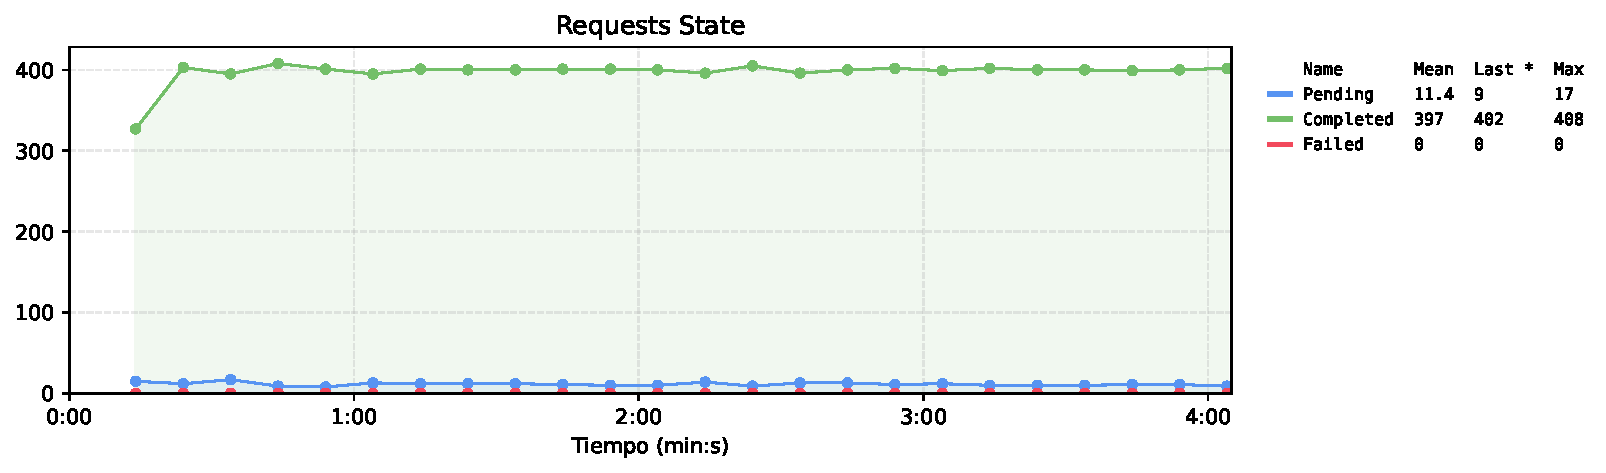
\includegraphics[width=\linewidth]{figures/sistema_base/baseline/requests_state}
                \end{minipage}%
                \hfill
                \begin{minipage}[c]{0.45\columnwidth}
                    Para evaluar la disponibilidad del sistema monitoreamos el estado de las request.
                    El eje $x$ muestra el tiempo transcurrido de la prueba y cada punto agrupa una ventana de 10 segundos.
                    Completed indica cuántas requests finalizaron correctamente en esa ventana, mientras que Pending indica cuántas seguían en curso.
                    Adicionalmente en la leyenda de la derecha se muestra el promedio, el ultimo valor y el maximo.\\
                    En 4 minutos con una carga de 40 request por segundo, se puede observar que el sistema no presento inconvenientes.
                \end{minipage}
                \label{fig:sistema_base_baseline_requests_state}
            \end{figure}

        \subsubsection{Latencia}
        \label{sec:sistema_base_pruebas_de_baseline_metricas_latencia}

            \begin{figure}[H]
                \centering
                \begin{minipage}[c]{0.5\columnwidth}
                    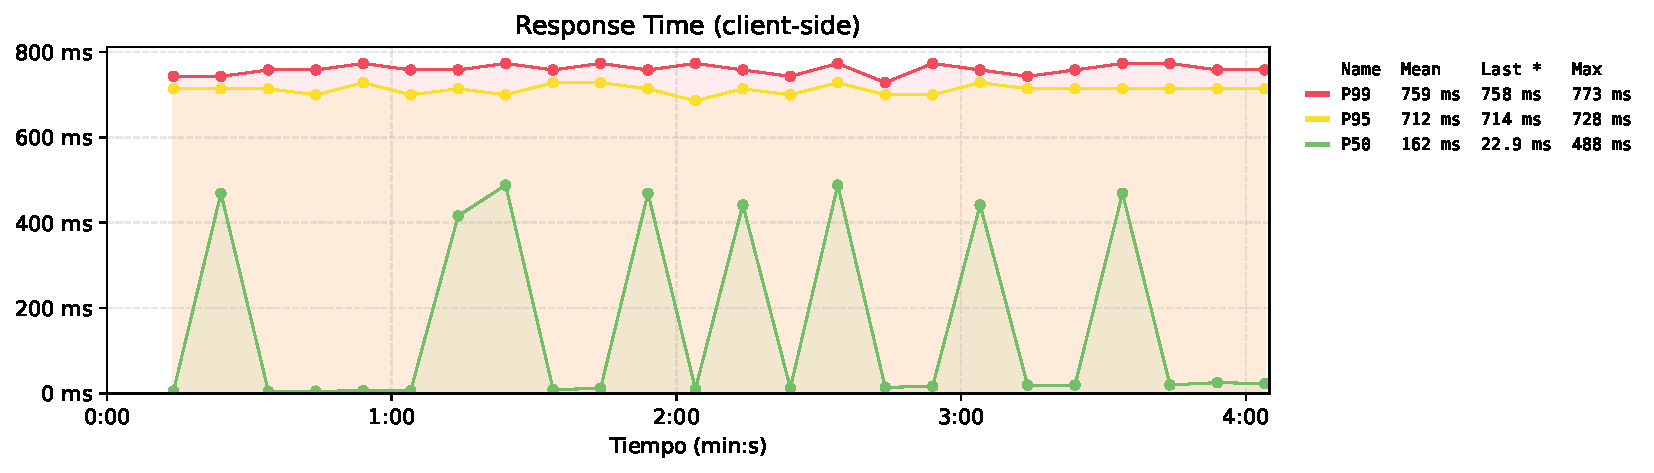
\includegraphics[width=\linewidth]{figures/sistema_base/baseline/response_time}
                \end{minipage}%
                \hfill
                \begin{minipage}[c]{0.45\columnwidth}
                    Para evaluar la latencia del sistema optamos por utilizar dos metodologias, la primera monitorear los tiempos de respuestas desde la perspectiva del cliente a travez de Artillery.
                    Optamos por realizar el monitoreo en P50, P95 Y P99, sinembargo una consideracion importante para esta metodlogia es que no distingue entre endpoints.
                    Se mantiene el formato de tiempo en el eje $x$ con ventanas de 10 segundos.
                \end{minipage}
                \label{fig:sistema_base_baseline_response_time}
            \end{figure}

            \begin{figure}[H]
                \centering
                \begin{minipage}[c]{0.5\columnwidth}
                    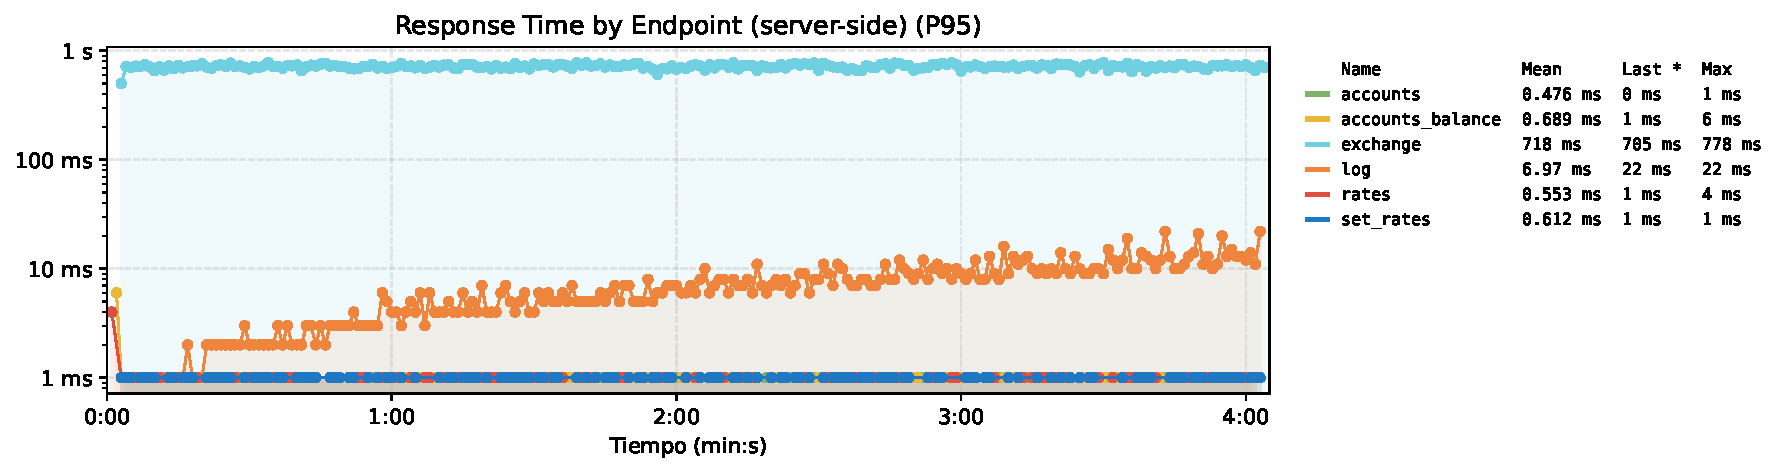
\includegraphics[width=\linewidth]{figures/sistema_base/baseline/endpoint_response_time}
                \end{minipage}%
                \hfill
                \begin{minipage}[c]{0.45\columnwidth}
                    La siguiente metodologia adoptada fue medir los tiempos de respuesta por endpoint desde la perspectiva del servidor.
                    Se realizo agregando la recoleccion de metricas directamente en el servidor.
                    Si bien en contraposicion a la metodologia anterior si podemos discernir entre endpoints, optamos por representarlo solo para P95 para no saturar la representacion.
                    Se mantiene el formato de tiempo en el eje $x$ con ventanas de 10 segundos, sinembargo para el eje $y$ optamos por una escala logaritmica por la gran discrepancia entre los tiempos.
                \end{minipage}
                \label{fig:sistema_base_baseline_endpoint_response_time}
            \end{figure}

        \subsubsection{Uso de recursos}
        \label{sec:sistema_base_pruebas_de_baseline_metricas_recursos}

            \begin{figure}[H]
                \centering
                \begin{minipage}[c]{0.5\columnwidth}
                    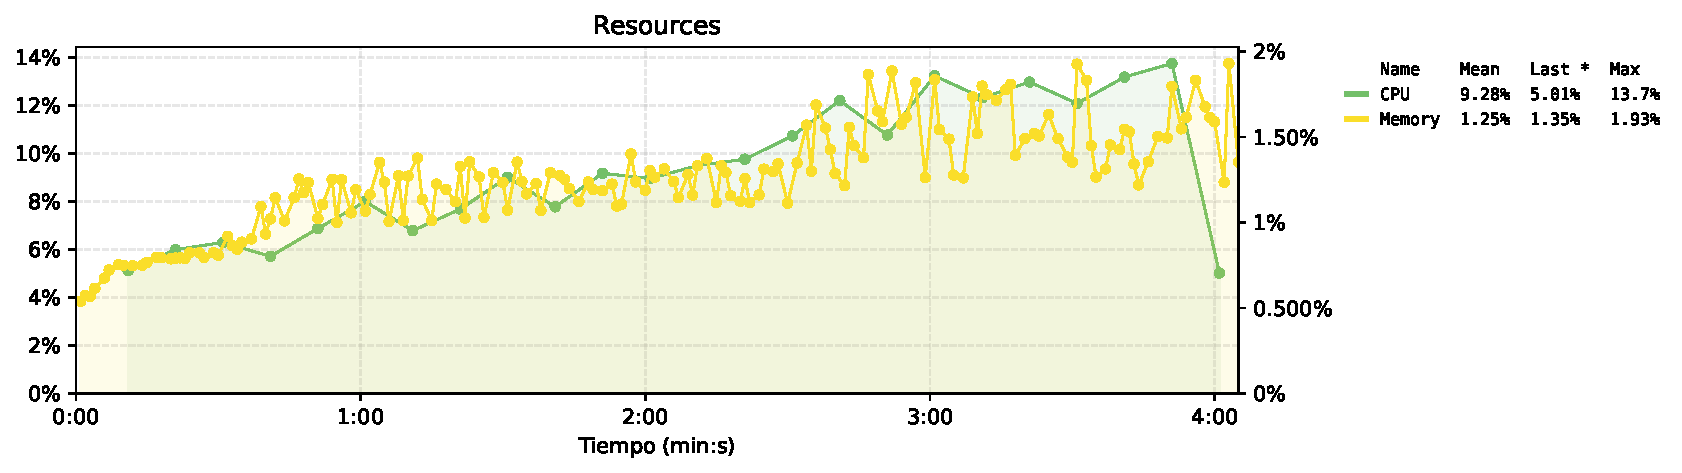
\includegraphics[width=\linewidth]{figures/sistema_base/baseline/resources}
                \end{minipage}%
                \hfill
                \begin{minipage}[c]{0.45\columnwidth}
                    Para evaluar el uso de recursos del sistema, monitoreamos el uso del CPU y de la memoria.
                    El uso del CPU se lee sobre el eje $y$ al lado izquierdo mientras que el uso de la memoria al lado derecho.
                    Nuevamente, mantiene el formato de tiempo en el eje $x$ con ventanas de 10 segundos.
                \end{minipage}
                \label{fig:sistema_base_baseline_resources}
            \end{figure}

        \subsubsection{Volumen operado por moneda}
        \label{sec:sistema_base_pruebas_de_baseline_metricas_volumen_operado_por_moneda}

            \begin{figure}[H]
                \centering
                \begin{minipage}[c]{0.5\columnwidth}
                    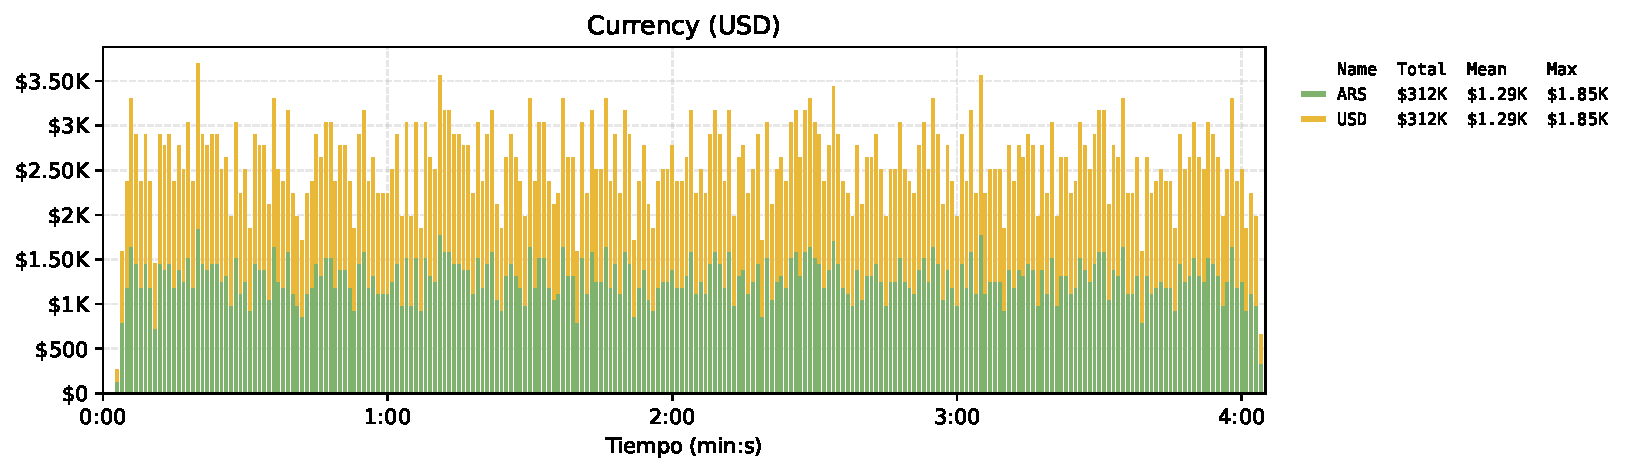
\includegraphics[width=\linewidth]{figures/sistema_base/baseline/currency}
                \end{minipage}%
                \hfill
                \begin{minipage}[c]{0.45\columnwidth}
                    Como la primera metrica de negocio, se evaluo el volumen operado por cada moneda.
                    Para esto se agrego la recoleccion de metricas directamente en el servidor.
                    Optamos por representar cada moneda con su respectivo valor en dolares, a la cotizacion vigente en cada operacion, para que los valores sean comparables.
                    Los volumenes de diferentes monedas operados en un mismo punto se apilan para representar el total operado en ese punto.
                    Se mantiene el formato de tiempo en el eje $x$ pero se redujo la ventana a 1 segundo.
                \end{minipage}
                \label{fig:sistema_base_baseline_currency}
            \end{figure}

        \subsubsection{Volumen neto operado}
        \label{sec:sistema_base_pruebas_de_baseline_metricas_volumen_neto_operado_por_moneda}

            \begin{figure}[H]
                \centering
                \begin{minipage}[c]{0.5\columnwidth}
                    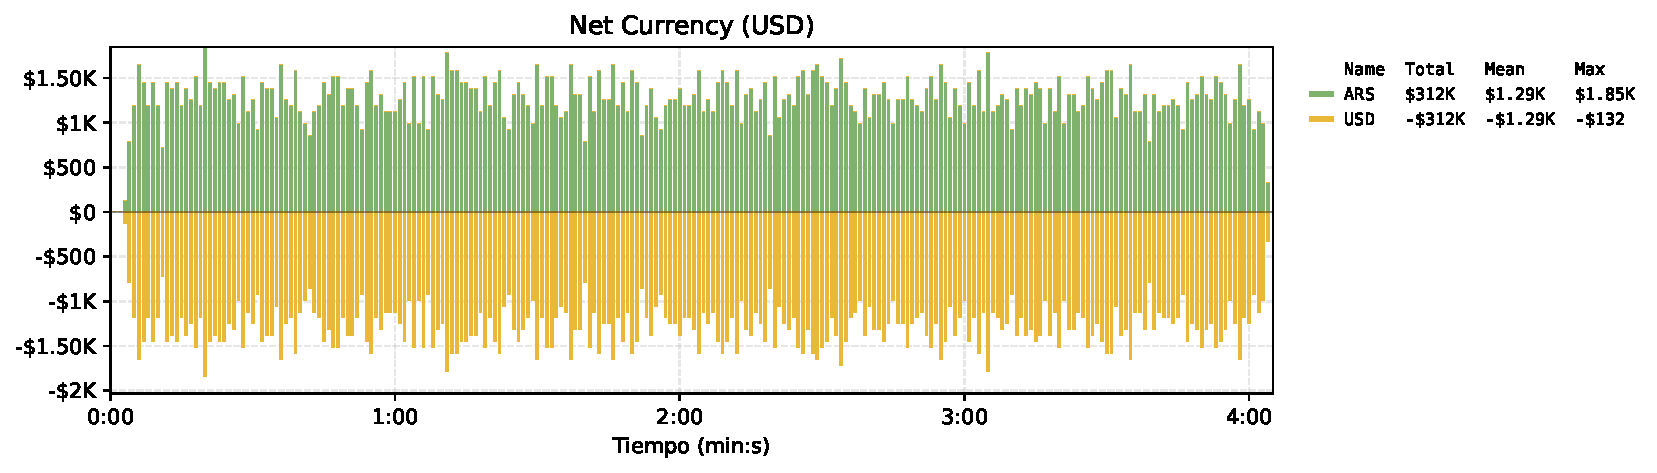
\includegraphics[width=\linewidth]{figures/sistema_base/baseline/net_currency}
                \end{minipage}%
                \hfill
                \begin{minipage}[c]{0.45\columnwidth}
                    Para la segunda metrica de negocio, se evaluo el volumen neto operado por cada moneda.
                    Nuevamente, a travez de la recoleccion de metricas directamente en el servidor.
                    De igual modo, con cada moneda en su respectivo valor en dolares.
                    A diferencia del volumen operado, las ventas se representan como valores negativos y las compras con valores positivos.
                    Se mantiene el formato de tiempo en el eje $x$ y la ventana de 1 segundo.
                \end{minipage}
                \label{fig:sistema_base_baseline_net_currency}
            \end{figure}

    \subsection{Pruebas de estrés}
    \label{sec:sistema_base_pruebas_de_stress}

        La prueba de estrés se realizo incrementando progresivamente la carga desde 40 hasta 180 en saltos de 20, cada salto con una duracion de 45s, el tiempo total de la prueba es de 450s (7,5 minutos).
        Se realizo un warm-up inicial de 5 usuarios durante 30s. Ademas, al final de la prueba se dejo una instancia de recovery de nuevamente 5 usuarios esta vez durante 60s.
        Tampoco se realizaron recargas de saldo intermedias y se mantuvo el mismo uso de endpoints para que los resultados sean comparables.

        Se pueden encontrar los resultados completos en el \hyperref[sec:resultados_completos_sistema_base_stress]{Apendice}.

        \subsubsection{Disponibilidad}
        \label{sec:sistema_base_pruebas_de_stress_metricas_disponibilidad}

            \begin{figure}[H]
                \centering
                \begin{minipage}[c]{0.5\columnwidth}
                    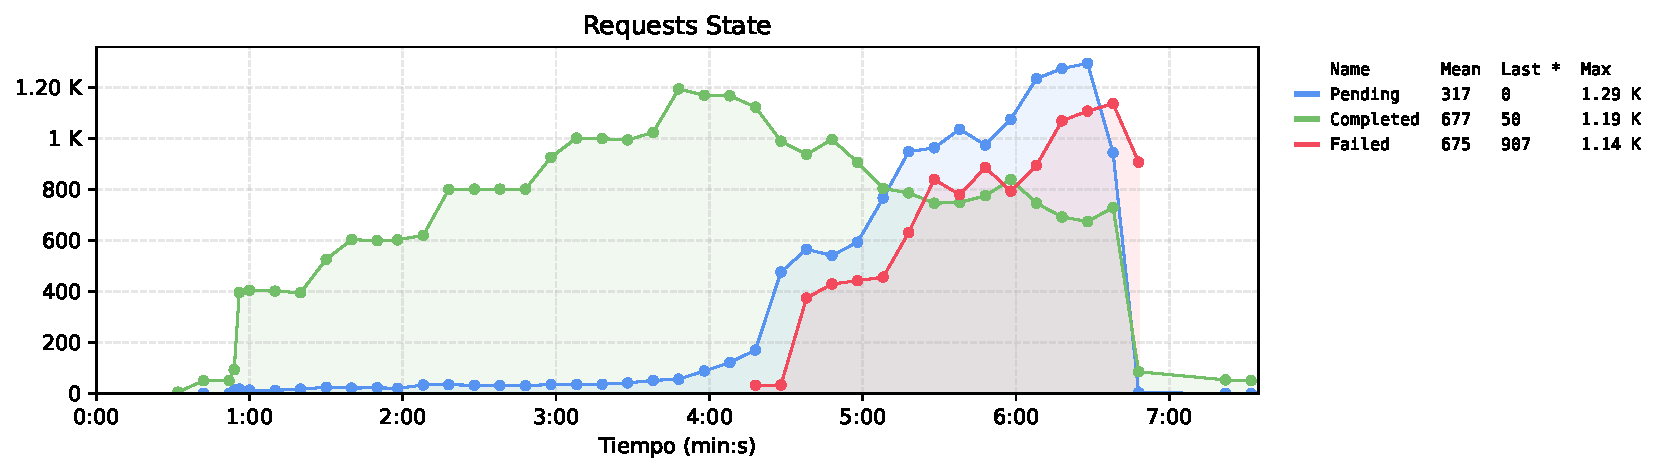
\includegraphics[width=\linewidth]{figures/sistema_base/stress/requests_state}
                \end{minipage}%
                \hfill
                \begin{minipage}[c]{0.45\columnwidth}
                    \todo{completar}
                \end{minipage}
                \label{fig:sistema_base_stress_requests_state}
            \end{figure}

        \subsubsection{Latencia}
        \label{sec:sistema_base_pruebas_de_stress_metricas_latencia}

            \begin{figure}[H]
                \centering
                \begin{minipage}[c]{0.5\columnwidth}
                    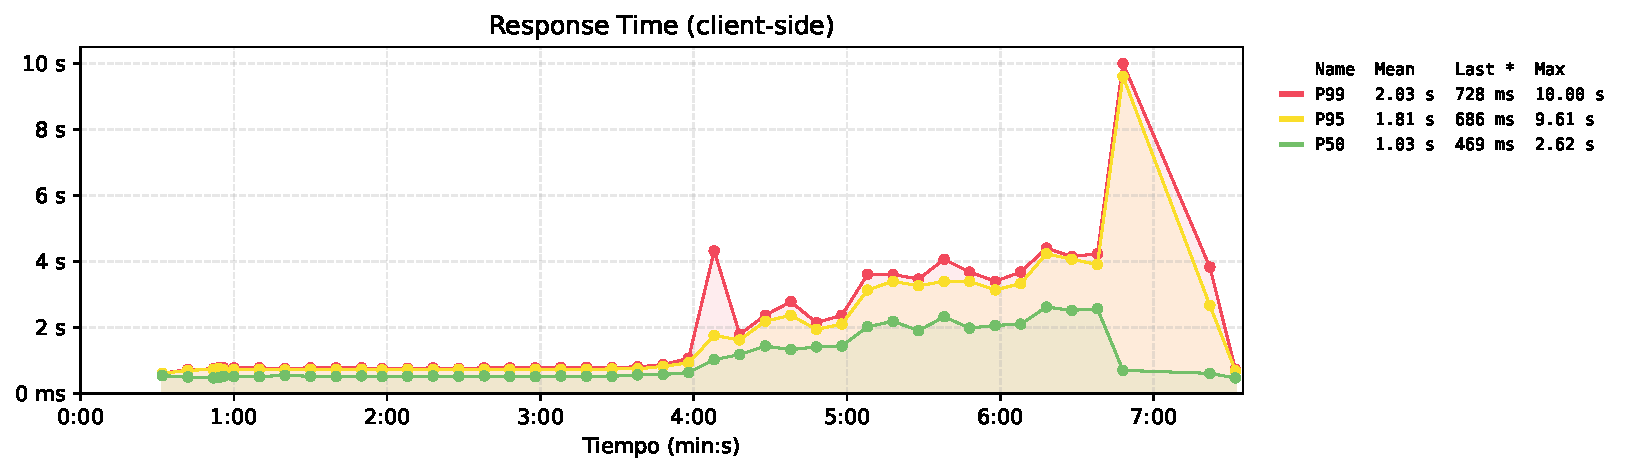
\includegraphics[width=\linewidth]{figures/sistema_base/stress/response_time}
                \end{minipage}%
                \hfill
                \begin{minipage}[c]{0.45\columnwidth}
                    \todo{completar}
                \end{minipage}
                \label{fig:sistema_base_stress_response_time}
            \end{figure}

            \begin{figure}[H]
                \centering
                \begin{minipage}[c]{0.5\columnwidth}
                    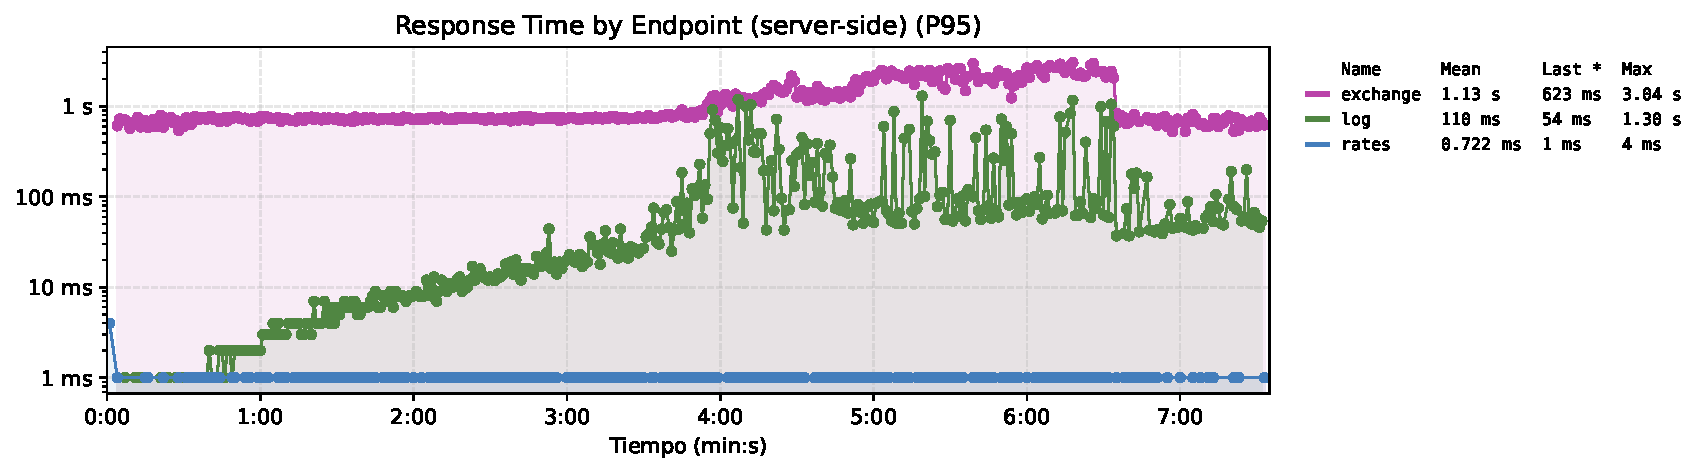
\includegraphics[width=\linewidth]{figures/sistema_base/stress/endpoint_response_time}
                \end{minipage}%
                \hfill
                \begin{minipage}[c]{0.45\columnwidth}
                    \todo{completar}
                \end{minipage}
                \label{fig:sistema_base_stress_endpoint_response_time}
            \end{figure}

        \subsubsection{Uso de recursos}
        \label{sec:sistema_base_pruebas_de_stress_metricas_recursos}

            \begin{figure}[H]
                \centering
                \begin{minipage}[c]{0.5\columnwidth}
                    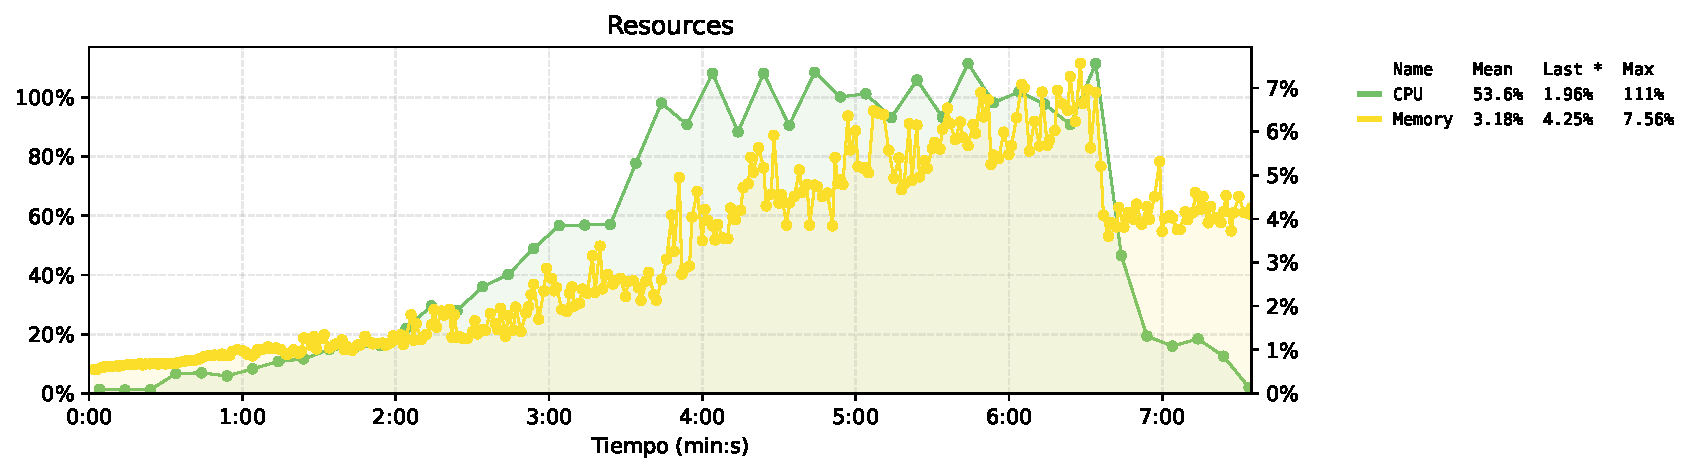
\includegraphics[width=\linewidth]{figures/sistema_base/stress/resources}
                \end{minipage}%
                \hfill
                \begin{minipage}[c]{0.45\columnwidth}
                    \todo{completar}
                \end{minipage}
                \label{fig:sistema_base_stress_resources}
            \end{figure}

        \subsubsection{Volumen operado por moneda}
        \label{sec:sistema_base_pruebas_de_stress_metricas_volumen_operado_por_moneda}

            \begin{figure}[H]
                \centering
                \begin{minipage}[c]{0.5\columnwidth}
                    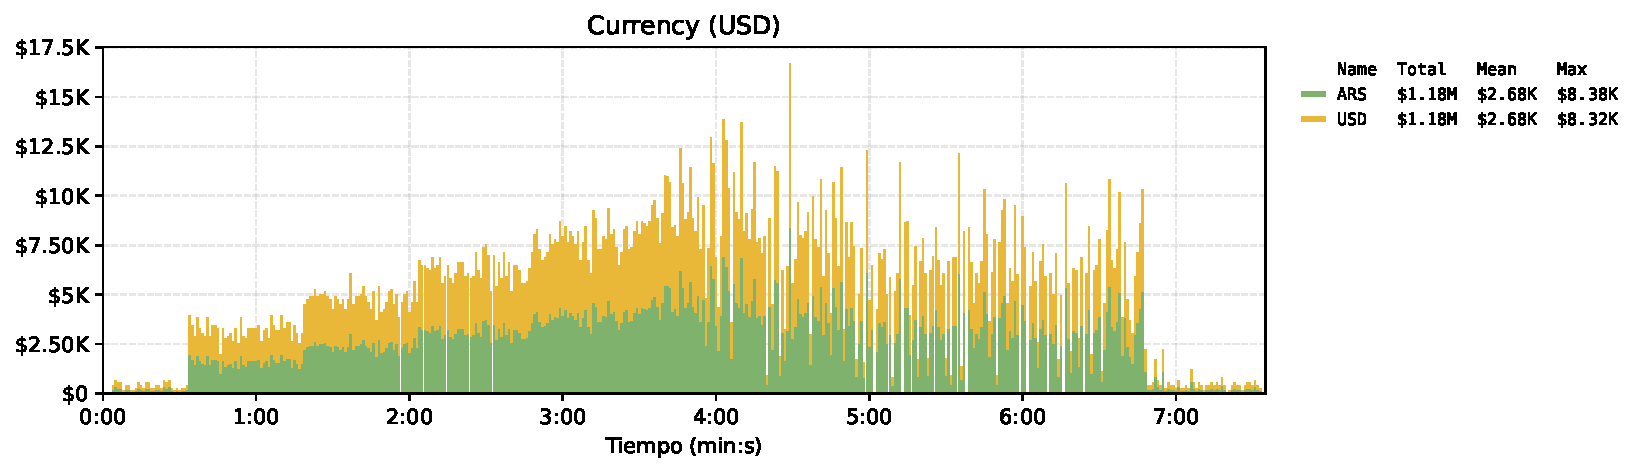
\includegraphics[width=\linewidth]{figures/sistema_base/stress/currency}
                \end{minipage}%
                \hfill
                \begin{minipage}[c]{0.45\columnwidth}
                    \todo{completar}
                \end{minipage}
                \label{fig:sistema_base_stress_currency}
            \end{figure}

        \subsubsection{Volumen neto operado}
        \label{sec:sistema_base_pruebas_de_stress_metricas_volumen_neto_operado_por_moneda}

            \begin{figure}[H]
                \centering
                \begin{minipage}[c]{0.5\columnwidth}
                    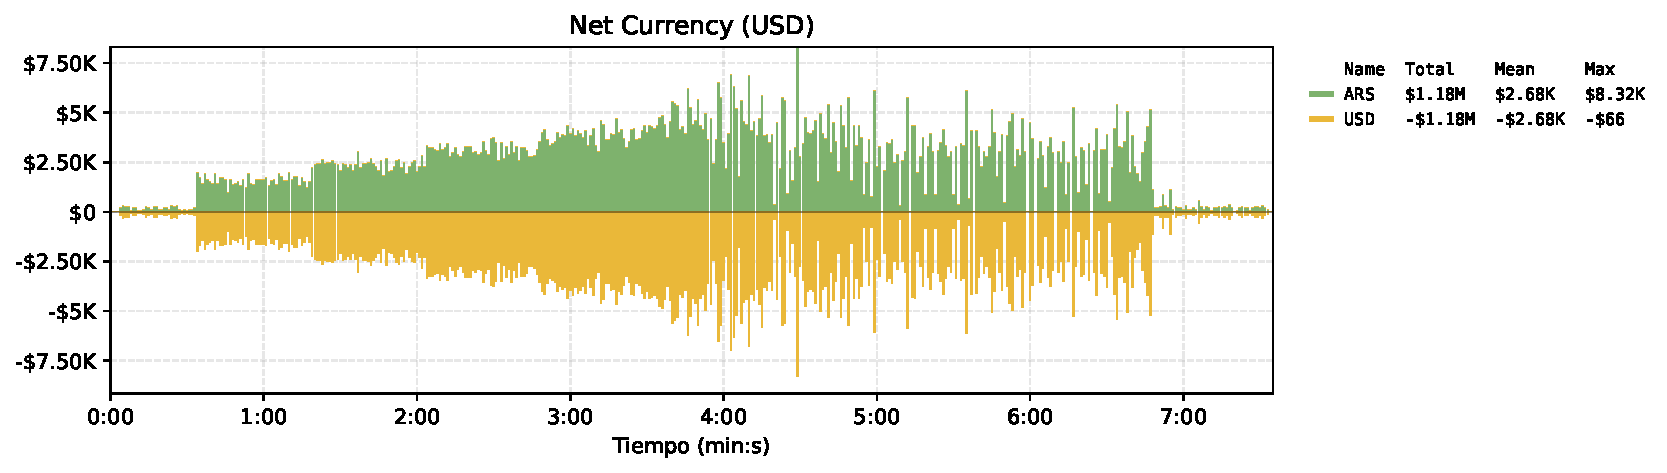
\includegraphics[width=\linewidth]{figures/sistema_base/stress/net_currency}
                \end{minipage}%
                \hfill
                \begin{minipage}[c]{0.45\columnwidth}
                    \todo{completar}
                \end{minipage}
                \label{fig:sistema_base_stress_net_currency}
            \end{figure}

    \subsection{Pruebas de resistencia}
    \label{sec:sistema_base_pruebas_de_soak}

    Se pueden encontrar los resultados completos en el \hyperref[sec:resultados_completos_sistema_base_soak]{Apendice}.

        \subsubsection{Disponibilidad}
        \label{sec:sistema_base_pruebas_de_soak_metricas_disponibilidad}

            \begin{figure}[H]
                \centering
                \begin{minipage}[c]{0.5\columnwidth}
                    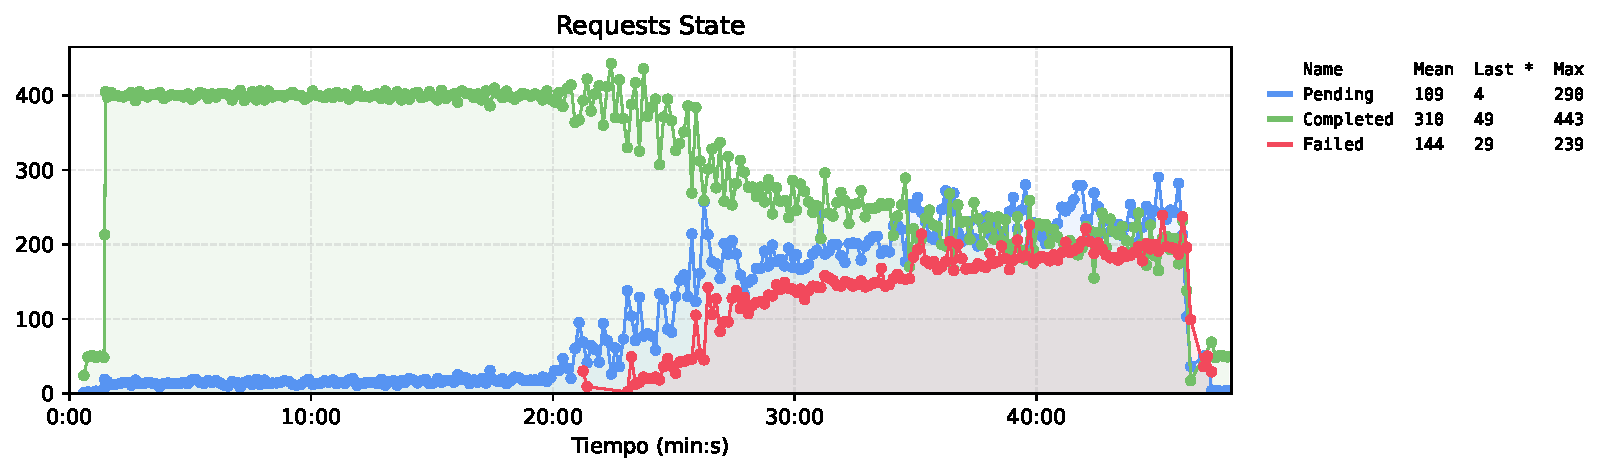
\includegraphics[width=\linewidth]{figures/sistema_base/soak/requests_state}
                \end{minipage}%
                \hfill
                \begin{minipage}[c]{0.45\columnwidth}
                    \todo{completar}
                \end{minipage}
                \label{fig:sistema_base_soak_requests_state}
            \end{figure}

        \subsubsection{Latencia}
        \label{sec:sistema_base_pruebas_de_soak_metricas_latencia}

            \begin{figure}[H]
                \centering
                \begin{minipage}[c]{0.5\columnwidth}
                    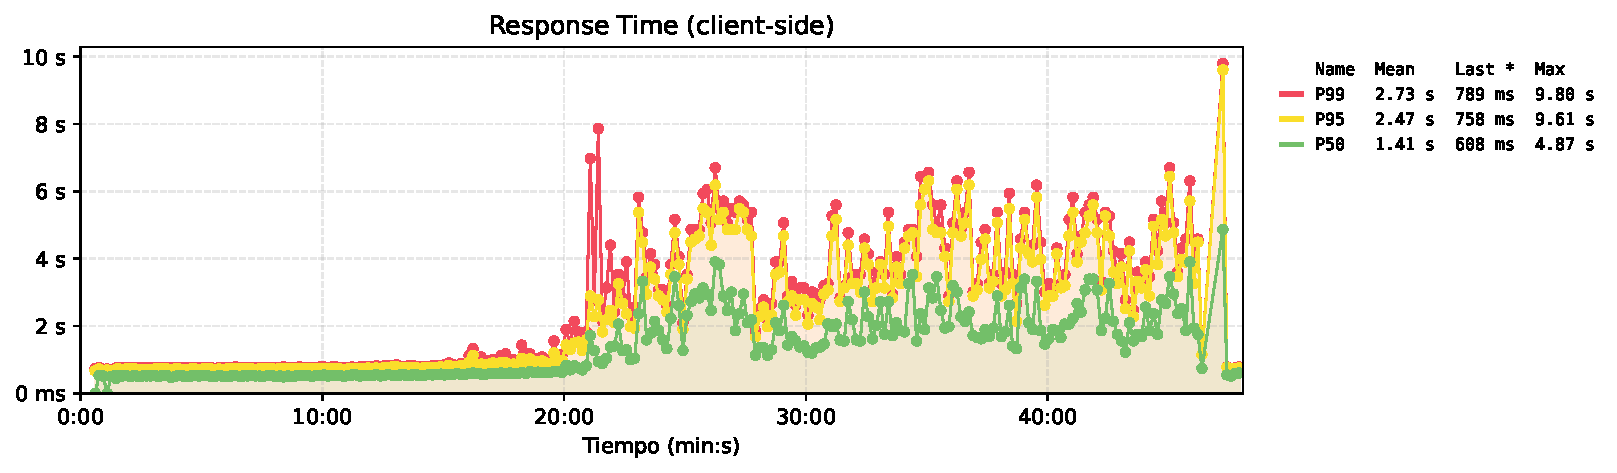
\includegraphics[width=\linewidth]{figures/sistema_base/soak/response_time}
                \end{minipage}%
                \hfill
                \begin{minipage}[c]{0.45\columnwidth}
                    \todo{completar}
                \end{minipage}
                \label{fig:sistema_base_soak_response_time}
            \end{figure}

            \begin{figure}[H]
                \centering
                \begin{minipage}[c]{0.5\columnwidth}
                    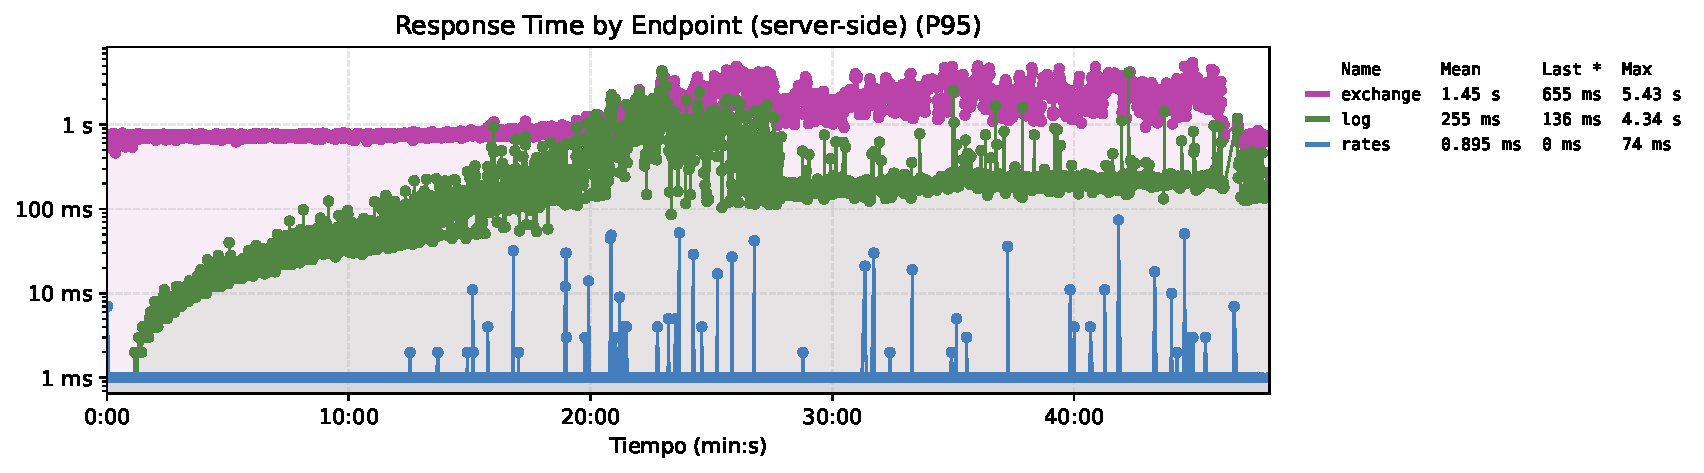
\includegraphics[width=\linewidth]{figures/sistema_base/soak/endpoint_response_time}
                \end{minipage}%
                \hfill
                \begin{minipage}[c]{0.45\columnwidth}
                    \todo{completar}
                \end{minipage}
                \label{fig:sistema_base_soak_endpoint_response_time}
            \end{figure}

        \subsubsection{Uso de recursos}
        \label{sec:sistema_base_pruebas_de_soak_metricas_recursos}

            \begin{figure}[H]
                \centering
                \begin{minipage}[c]{0.5\columnwidth}
                    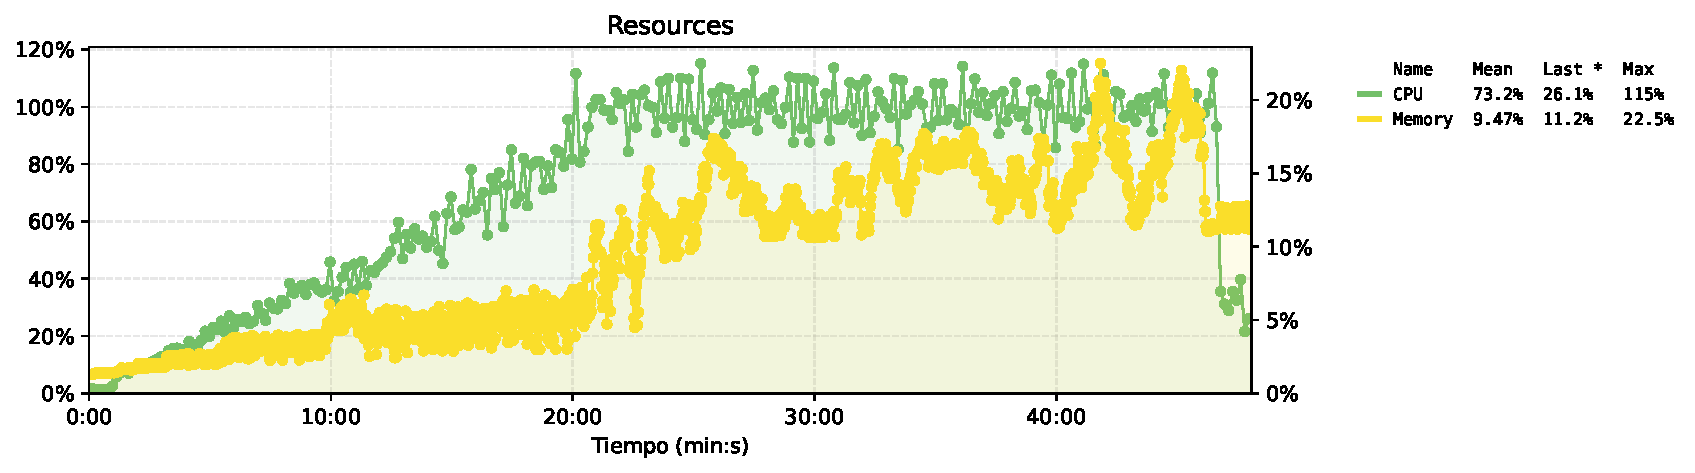
\includegraphics[width=\linewidth]{figures/sistema_base/soak/resources}
                \end{minipage}%
                \hfill
                \begin{minipage}[c]{0.45\columnwidth}
                    \todo{completar}
                \end{minipage}
                \label{fig:sistema_base_soak_resources}
            \end{figure}

        \subsubsection{Volumen operado por moneda}
        \label{sec:sistema_base_pruebas_de_soak_metricas_volumen_operado_por_moneda}

            \begin{figure}[H]
                \centering
                \begin{minipage}[c]{0.5\columnwidth}
                    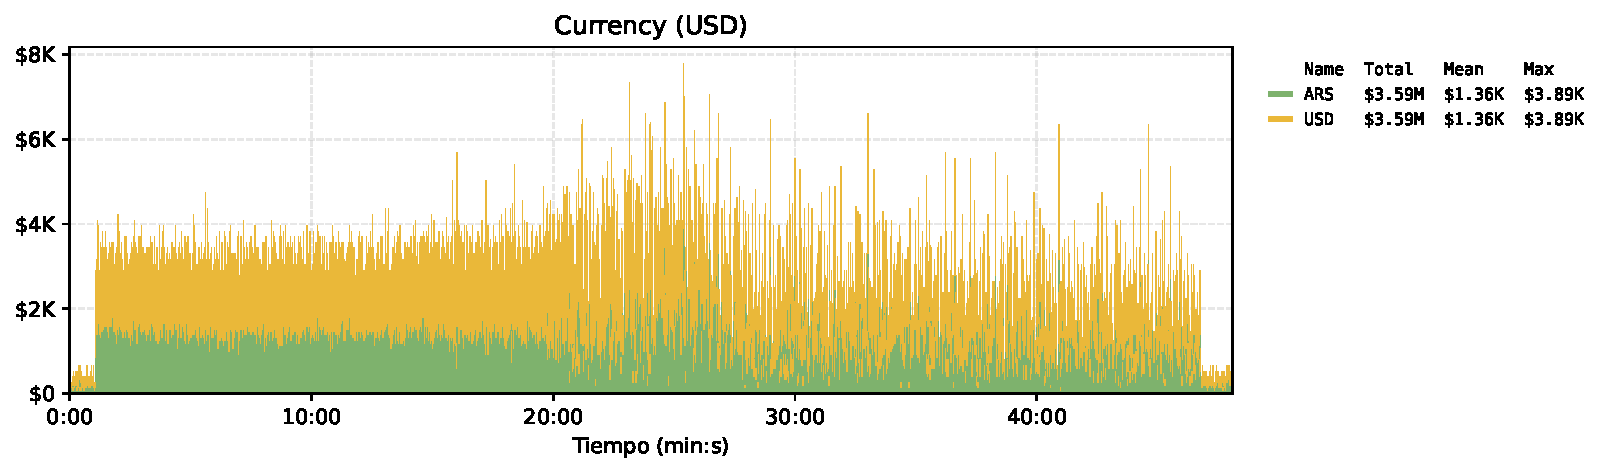
\includegraphics[width=\linewidth]{figures/sistema_base/soak/currency}
                \end{minipage}%
                \hfill
                \begin{minipage}[c]{0.45\columnwidth}
                    \todo{completar}
                \end{minipage}
                \label{fig:sistema_base_soak_currency}
            \end{figure}

        \subsubsection{Volumen neto operado}
        \label{sec:sistema_base_pruebas_de_soak_metricas_volumen_neto_operado_por_moneda}

            \begin{figure}[H]
                \centering
                \begin{minipage}[c]{0.5\columnwidth}
                    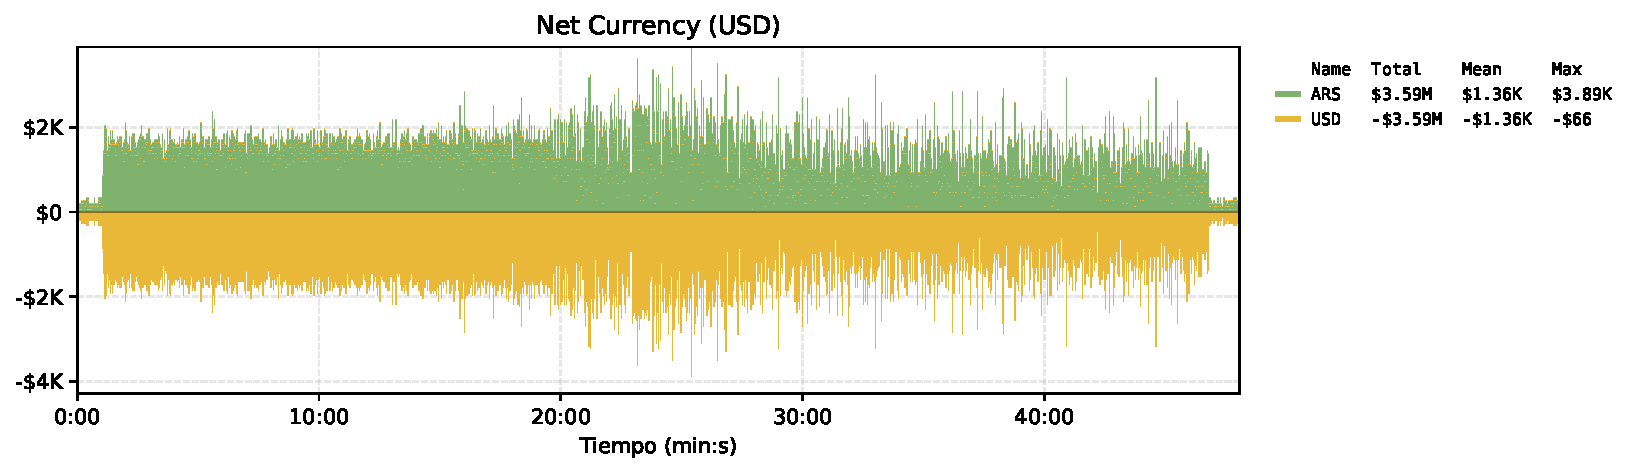
\includegraphics[width=\linewidth]{figures/sistema_base/soak/net_currency}
                \end{minipage}%
                \hfill
                \begin{minipage}[c]{0.45\columnwidth}
                    \todo{completar}
                \end{minipage}
                \label{fig:sistema_base_soak_net_currency}
            \end{figure}

    \subsection{Pruebas de caos}
    \label{sec:sistema_base_pruebas_de_chaos}

    Se pueden encontrar los resultados completos en el \hyperref[sec:resultados_completos_sistema_base_chaos]{Apendice}.

        \subsubsection{Disponibilidad}
        \label{sec:sistema_base_pruebas_de_chaos_metricas_disponibilidad}

            \begin{figure}[H]
                \centering
                \begin{minipage}[c]{0.5\columnwidth}
                    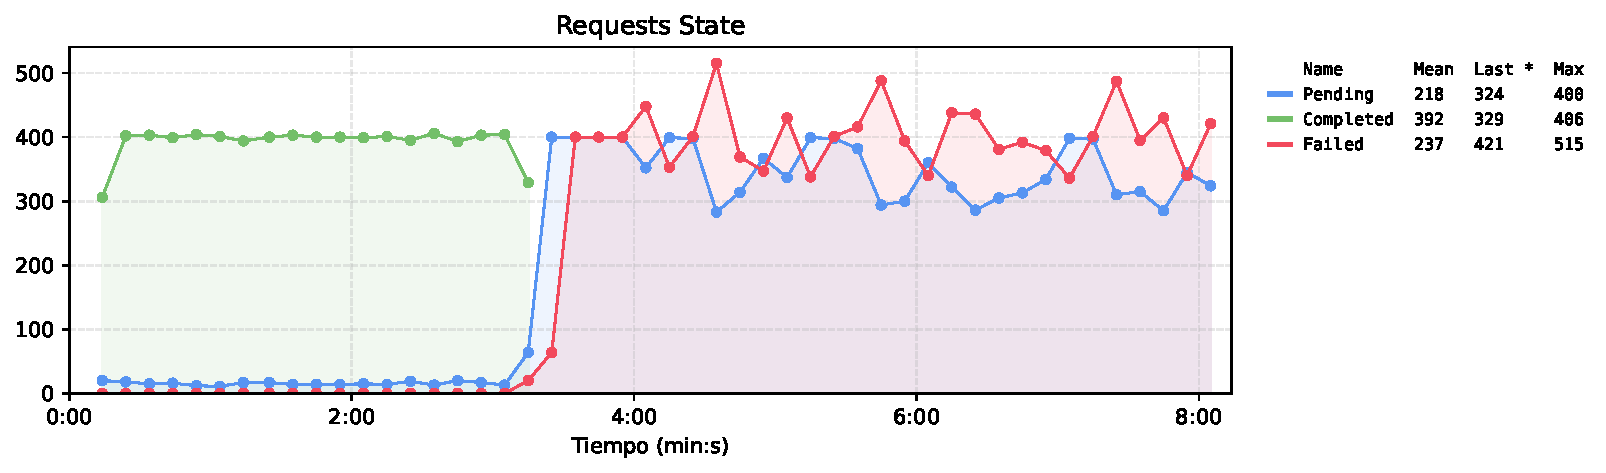
\includegraphics[width=\linewidth]{figures/sistema_base/chaos/requests_state}
                \end{minipage}%
                \hfill
                \begin{minipage}[c]{0.45\columnwidth}
                    \todo{completar}
                \end{minipage}
                \label{fig:sistema_base_chaos_requests_state}
            \end{figure}

        \subsubsection{Latencia}
        \label{sec:sistema_base_pruebas_de_chaos_metricas_latencia}

            \begin{figure}[H]
                \centering
                \begin{minipage}[c]{0.5\columnwidth}
                    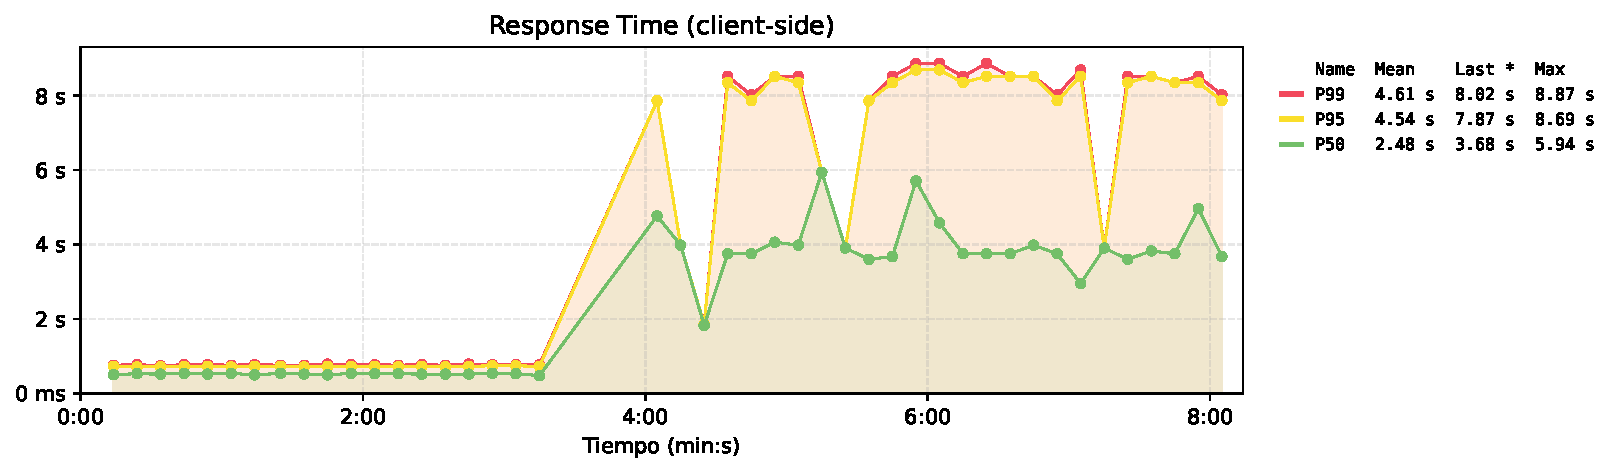
\includegraphics[width=\linewidth]{figures/sistema_base/chaos/response_time}
                \end{minipage}%
                \hfill
                \begin{minipage}[c]{0.45\columnwidth}
                    \todo{completar}
                \end{minipage}
                \label{fig:sistema_base_chaos_response_time}
            \end{figure}

            \begin{figure}[H]
                \centering
                \begin{minipage}[c]{0.5\columnwidth}
                    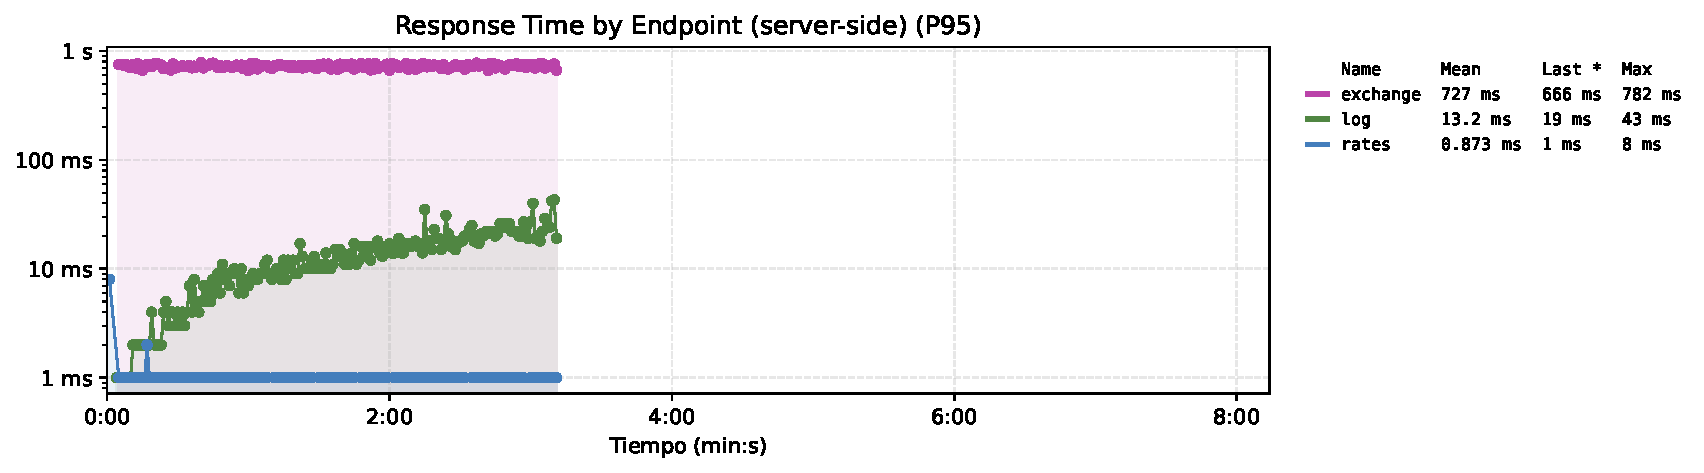
\includegraphics[width=\linewidth]{figures/sistema_base/chaos/endpoint_response_time}
                \end{minipage}%
                \hfill
                \begin{minipage}[c]{0.45\columnwidth}
                    \todo{completar}
                \end{minipage}
                \label{fig:sistema_base_chaos_endpoint_response_time}
            \end{figure}

        \subsubsection{Uso de recursos}
        \label{sec:sistema_base_pruebas_de_chaos_metricas_recursos}

            \begin{figure}[H]
                \centering
                \begin{minipage}[c]{0.5\columnwidth}
                    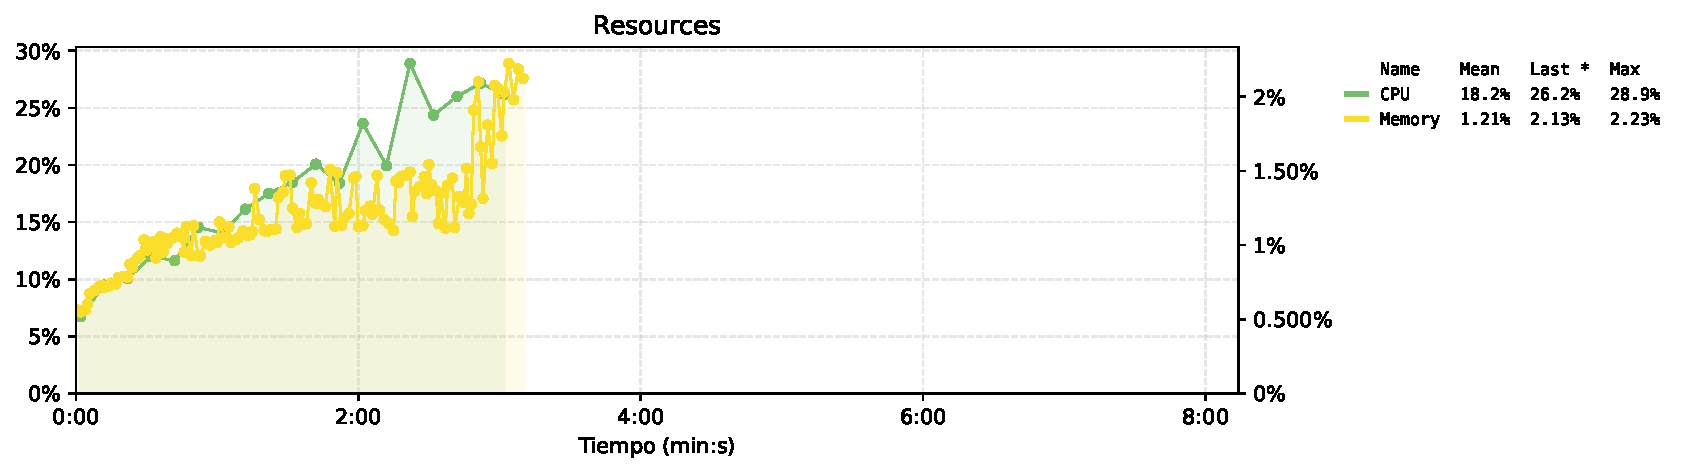
\includegraphics[width=\linewidth]{figures/sistema_base/chaos/resources}
                \end{minipage}%
                \hfill
                \begin{minipage}[c]{0.45\columnwidth}
                    \todo{completar}
                \end{minipage}
                \label{fig:sistema_base_chaos_resources}
            \end{figure}

        \subsubsection{Volumen operado por moneda}
        \label{sec:sistema_base_pruebas_de_chaos_metricas_volumen_operado_por_moneda}

            \begin{figure}[H]
                \centering
                \begin{minipage}[c]{0.5\columnwidth}
                    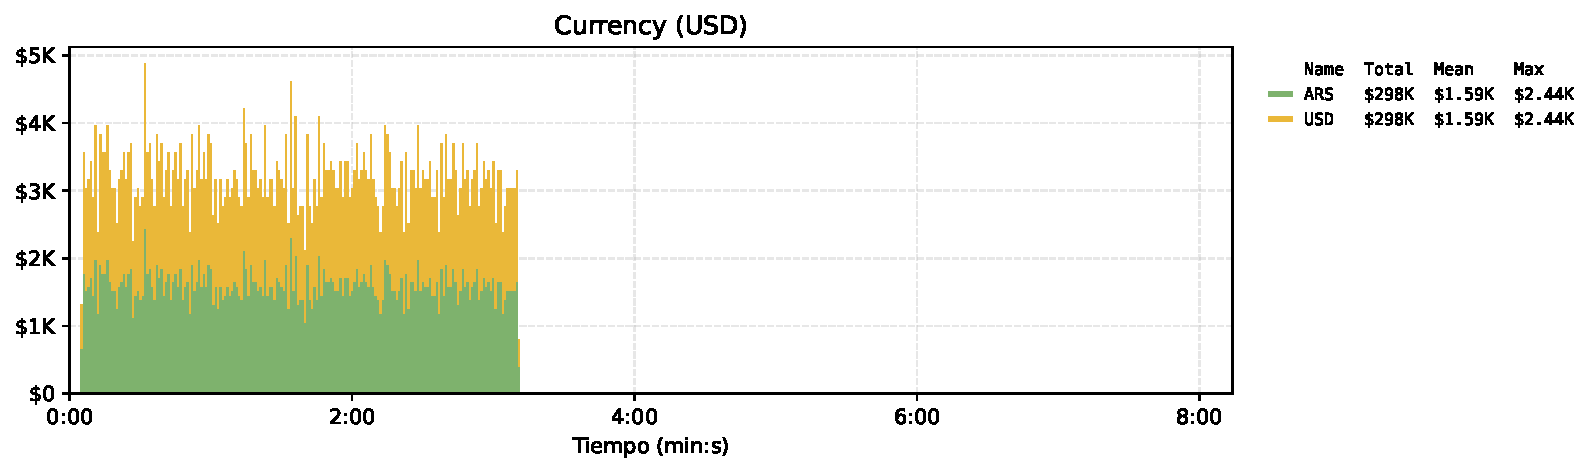
\includegraphics[width=\linewidth]{figures/sistema_base/chaos/currency}
                \end{minipage}%
                \hfill
                \begin{minipage}[c]{0.45\columnwidth}
                    \todo{completar}
                \end{minipage}
                \label{fig:sistema_base_chaos_currency}
            \end{figure}

        \subsubsection{Volumen neto operado}
        \label{sec:sistema_base_pruebas_de_chaos_metricas_volumen_neto_operado_por_moneda}

            \begin{figure}[H]
                \centering
                \begin{minipage}[c]{0.5\columnwidth}
                    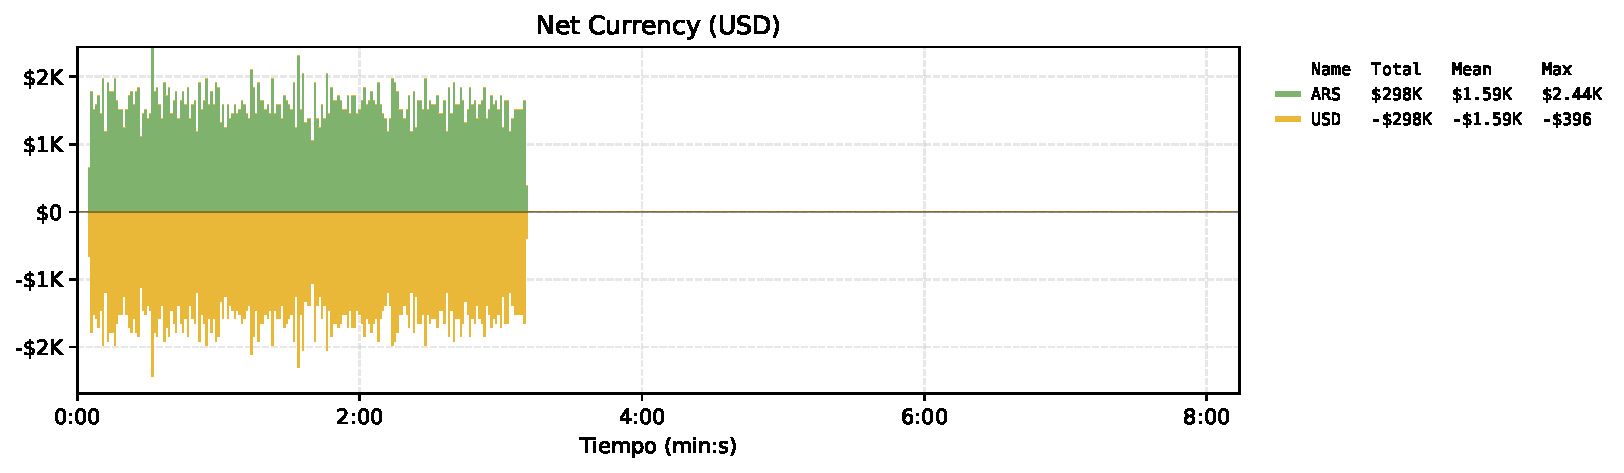
\includegraphics[width=\linewidth]{figures/sistema_base/chaos/net_currency}
                \end{minipage}%
                \hfill
                \begin{minipage}[c]{0.45\columnwidth}
                    \todo{completar}
                \end{minipage}
                \label{fig:sistema_base_chaos_net_currency}
            \end{figure}
